% Copyright 2004 by Till Tantau <tantau@users.sourceforge.net>.
%
% In principle, this file can be redistributed and/or modified under
% the terms of the GNU Public License, version 2.
%
% However, this file is supposed to be a template to be modified
% for your own needs. For this reason, if you use this file as a
% template and not specifically distribute it as part of a another
% package/program, I grant the extra permission to freely copy and
% modify this file as you see fit and even to delete this copyright
% notice. 

\documentclass{beamer}

\usepackage[utf8]{inputenc}
\usepackage[T1]{fontenc}
\usepackage{graphicx}
\usepackage{tikz}
\usepackage{caption}
\usepackage{amssymb}
\usepackage{amsmath}


% There are many different themes available for Beamer. A comprehensive
% list with examples is given here:
% http://deic.uab.es/~iblanes/beamer_gallery/index_by_theme.html
% You can uncomment the themes below if you would like to use a different
% one:
%\usetheme{AnnArbor}
%\usetheme{Antibes}
%\usetheme{Bergen}
%\usetheme{Berkeley}
%\usetheme{Berlin}
%\usetheme{Boadilla}
%\usetheme{boxes}
%\usetheme{CambridgeUS}
%\usetheme{Copenhagen}
%\usetheme{Darmstadt}
%\usetheme{default}
%\usetheme{Frankfurt}
%\usetheme{Goettingen}
%\usetheme{Hannover}
%\usetheme{Ilmenau}
%\usetheme{JuanLesPins}
%\usetheme{Luebeck}
%\usetheme{Madrid}
%\usetheme{Malmoe}
%\usetheme{Marburg}
\usetheme{Montpellier}
%\usetheme{PaloAlto}
%\usetheme{Pittsburgh}
%\usetheme{Rochester}
%\usetheme{Singapore}
%\usetheme{Szeged}
%\usetheme{Warsaw}

\title{\bf{The Search for Simple Systems}}

% A subtitle is optional and this may be deleted
\subtitle{Genetic Information, Autocatalytic Sets}

\author{Alex Popinga and Peter Wills (UoA)} %\\ feat. Lloyd Sanders (UoA), Federico Paoletti and Jotun Hein (Oxford)}
% - Give the names in the same order as the appear in the paper.
% - Use the \inst{?} command only if the authors have different
%   affiliation.

%\institute[Universities of Somewhere and Elsewhere] % (optional, but mostly needed)
{
%\begin{figure}
%\includegraphics[width=0.6\linewidth]{RAF01.png}

%\tiny{``Plague Inc." (Ndemic Creations)}
%\end{figure}
}
  
% - Use the \inst command only if there are several affiliations.
% - Keep it simple, no one is interested in your street address.

\date{\small{\textit{New Zealand Astrobiology Initiative Workshop, 2016}}}
% - Either use conference name or its abbreviation.
% - Not really informative to the audience, more for people (including
%   yourself) who are reading the slides online

%\subject{Theoretical Computer Science}
% This is only inserted into the PDF information catalog. Can be left
% out. 

% If you have a file called "university-logo-filename.xxx", where xxx
% is a graphic format that can be processed by latex or pdflatex,
% resp., then you can add a logo as follows:

% \pgfdeclareimage[height=0.5cm]{university-logo}{university-logo-filename}
% \logo{\pgfuseimage{university-logo}}

% Delete this, if you do not want the table of contents to pop up at
% the beginning of each subsection:
\AtBeginSubsection[]
{
  \begin{frame}<beamer>{Outline}
    \tableofcontents[currentsection,currentsubsection]
  \end{frame}
}

% Let's get started
\begin{document}

\usebackgroundtemplate%
{%
    \includegraphics[width=\paperwidth,height=\paperheight]{voyager1.jpg}%
}

\begin{frame}
  \titlepage
\end{frame}

\begin{frame}{Outline}
  \tableofcontents
  % You might wish to add the option [pausesections]
\end{frame}

\section{Genetic Information (and the "meaning" of life)}

\begin{frame}
\begin{itemize}
\item "flesti wonk ot somsoc eht rof yaw a era eW" 
\end{itemize}
\end{frame}

\begin{frame}
\begin{itemize}
\item "flesti wonk ot somsoc eht rof yaw a era eW" 
\end{itemize}

\begin{itemize}
\item \textbf{Sentence is reversed.}
\item Translation:  "We are a way for the cosmos to know itself" -Carl Sagan
\end{itemize}
\end{frame}

\begin{frame}
\begin{itemize}
\item "flesti wonk ot somsoc eht rof yaw a era eW" 
\end{itemize}

\begin{itemize}
\item \textbf{Sentence is reversed.}
\item Translation:  "We are a way for the cosmos to know itself" -Carl Sagan
\end{itemize}

\begin{itemize}
\item "flesti wonk ot" \textbf{means} "The"
\item "somsoc eht" \textbf{means} "meaning"
\item "rof yaw a era ew" \textbf{means} "of life is beer"
\item Translation:  "The meaning of life is beer" 
\end{itemize}
\end{frame}

%\begin{frame}
%"ttggaatctg aacaggacta gtagccacga gaatgagact cctaattcga gctgagcttg
%gacaacctgg aactcttcta ggagacgatc aaatttataa ttgccttatt accgctcatg
%gtctattaat gatatttttt gtagtcctac ctattttaat aggaggattt ggaaattgac"
%\vspace{6mm}
%\end{frame}

\begin{frame}
\vspace{7mm}
"ttggaatctg aacaggacta gtagccacga gaatgagact cctaattcga gctgagcttg
gacaacctgg aactcttcta ggagacgatc aaatttataa ttgccttatt accgctcatg
gtctattaat gatatttttt gtagtcctac ctattttaat aggaggattt ggaaattgac"

\vspace{3mm}
\begin{itemize}
\item Minimal information necessary?
\item Emergence?
\end{itemize}
\end{frame}


\begin{frame}
NASA Astrobiology Roadmap

\begin{itemize}
%\item "Understand the relationship between energy, information, and complexity."
\item  "Understand how molecules and systems, including emergent behavior and information transfer, depend on and scale with complexity."
\item "Identify the potential for creating catalytic and genetic functions."
\end{itemize}
\end{frame}

\section{Autocatalytic (RAF) Sets}

\begin{frame}
(Kauffman 1971) suggested that ``proto-organisms'' probably arose from chemical reaction systems, 
later elaborated as ``reflexively autocatalytic sets of peptides and polypeptides" (Kauffman 1986).

\vspace{5mm}
(Steel 2000) formalised Kauffman's "connected, reflexively autocatalytic" sets into RAF (reflexively autocatalytic, food-generated) set theory.
\end{frame}

%\begin{frame}
%Chemical reaction system (CRS) is defined as the tuple ($X$, $R$, $C$), where:

%\begin{itemize} 
%\item $X$ is the set of molecule types, 
%\item $R$ is the set of chemical reactions, and 
%\item $C$ is the catalytic set that describes which reactions are catalysed by which molecule types. (Hordijk 2015)
%\end{itemize}
%\end{frame}

\begin{frame}
Chemical reaction system (CRS) is defined as the tuple ($X$, $R$, $C$), where:

\begin{itemize} 
\item $X$ is the set of molecule types, 
\item $R$ is the set of chemical reactions, and 
\item $C$ is the catalytic set that describes which reactions are catalysed by which molecule types. (Hordijk 2015)
\end{itemize}

\vspace{3mm}
With a `food' set $F$ (subset of the molecules in $X$), the CRS becomes the quadruple $Q = (X, R, C, F)$.
\end{frame}


\begin{frame}
A subset of $R$, $R' \subseteq R$, is a RAF if it satisfies the following conditions:

\begin{itemize}
\item It is \textit{reflexively autocatalytic} %meaning that every reaction $r \in R'$ is catalysed by either a molecule in the food set $F$ or a molecule produced by one of a series of reactions starting with $F$.
\item It is \textit{food-generated} %meaning that for every reaction in $R'$ the reactant is either in the food set $F$ or can eventually be generated by a series of reactions starting with molecules in $F$.
\end{itemize}

%As described by (Kauffman 1986) and as done in previous RAF work (Hordijk 2004,Hordijk 2015), we choose a binary polymer model to explore the application of RAF theory to abstractions of information-carrying molecules in prebiotic systems.  

\end{frame}


\begin{frame}
\begin{figure}
%\begin{center}
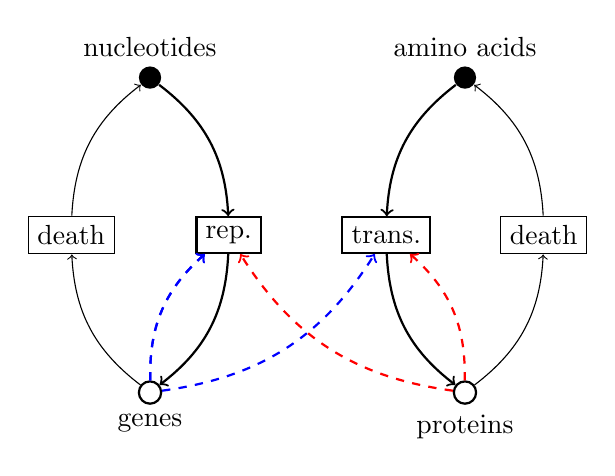
\begin{tikzpicture}

% genes node
\node[thick,circle, draw,inner sep=1mm] (genes) at (-2,0) {};
\node[below] at (genes.south) {genes};

% rep. reaction node
\node[thick,rectangle,draw] (r) at (-1,2) {rep.};

% nucleotides node
\node[circle, fill,inner sep=1mm] (nucleotides) at (-2,4) {};
\node[above] at (nucleotides.north) {nucleotides};

\draw[thick,->] (r) to [bend left=25] (genes);
\draw[thick,dashed,blue,->] (genes) to [bend left=25] (r);
\draw[thick,->] (nucleotides) to [bend left=25] (r);

% proteins node
\node[thick,circle, draw,inner sep=1mm] (proteins) at (2,0) {};
\node[below] at (proteins.south) {proteins};

% trans. reaction node
\node[thick,rectangle,draw] (t) at (1,2) {trans.};

% amino acids node
\node[circle, fill,inner sep=1mm] (amino acids) at (2,4) {};
\node[above] at (amino acids.north) {amino acids};

\draw[thick,->] (amino acids) to [bend right=25] (t);
\draw[thick,->] (t) to [bend right=25] (proteins);

\draw[thick,dashed,red,->] (proteins) to [bend left=25] (r);
\draw[thick,dashed,red,->] (proteins) to [bend right=25] (t);
\draw[thick,dashed,blue,->] (genes) to [bend left=25] (r);
\draw[thick,dashed,blue,->] (genes) to [bend right=25]  (t);

% genes degradation reaction node
\node[rectangle,draw] (genes death) at (-3,2) {death};

% genes diff reaction node
%\node[rectangle,draw] (genes diff) at (-5,-2) {diff[0$\rightharpoonup$1]};

% proteins degradation reaction node
\node[rectangle,draw] (proteins death) at (3,2) {death};

% proteins diff reaction node
%z\node[rectangle,draw] (proteins diff) at (5,-2) {diff[0$\rightharpoonup$1]};

\draw[->] (proteins death) to [bend right=25] (amino acids);
\draw[->] (proteins) to [bend right=25] (proteins death);

\draw[->] (genes death) to [bend left=25] (nucleotides);
\draw[->] (genes) to [bend left=25] (genes death);

\end{tikzpicture}
\end{figure}
\end{frame}

\section{The Gene-Replicase-Translatase (GRT) System}

\begin{frame}
\textbf{Minimal GRT molecule types}

\begin{itemize}
\item Nucleotides: $N = \{0,1\}$
\item Amino acids: $A = \{0,1\}$
\item Genes: $G = \{000, 001, 010, 011, \dots, 111\}$
\item Proteins: $P = \{000, 001, 010, 011, \dots, 111\}$
\end{itemize}

%In this primitive system we imagine a simple translation mechanism in which one `nucleotide' position in a gene is translated to one `amino acid' in a protein.  In other words, a codon is also represented by a single bit, and therefore a gene and its translated protein are always the same length.
\end{frame}


\begin{frame}
For evolution, there must be mutation! 

\begin{center}
AAACGTATTAG -> AAACGTATTAG

AAACGTATTAG -> AAACGTATTA\textcolor{red}{C}

\vspace{5mm}
$G_{010} \xrightarrow[]{P_{000}} G_{010} + G_{010}\quad \text{ at rate } \alpha_1
\label{eq:basicRep}$

$G_{010} \xrightarrow[]{P_{000}} G_{010} + G_{011}\quad \text{ at rate } \alpha_2
\label{eq:basicError}$

\end{center}
\end{frame}

\begin{frame}
\vspace{6mm}
For evolution, there must be mutation! 

\begin{center}
AAACGTATTAG -> AAACGTATTAG

AAACGTATTAG -> AAACGTATTA\textcolor{red}{C}

\vspace{5mm}
$G_{010} \xrightarrow[]{P_{000}} G_{010} + G_{010}\quad \text{ at rate } \alpha_1
\label{eq:basicRep}$

$G_{010} \xrightarrow[]{P_{000}} G_{010} + G_{011}\quad \text{ at rate } \alpha_2
\label{eq:basicError}$

\vspace{5mm}
$G_{010}[i] \xrightarrow[]{}G_{010}[j] \quad \text{ at rate } \gamma_2, \text{ with }|i-j|=1$
\end{center}
\end{frame}

\begin{frame}
\begin{figure}
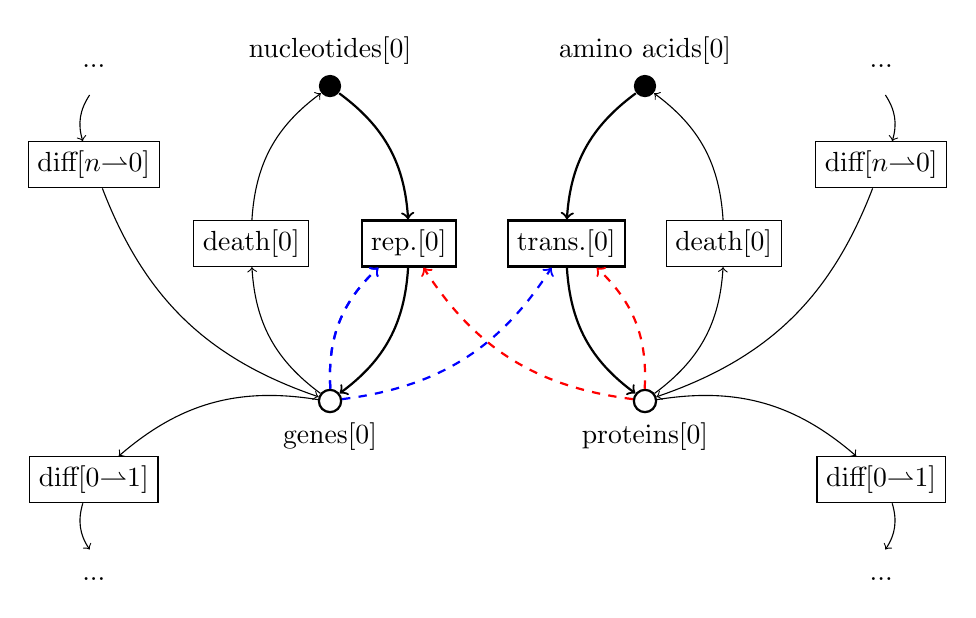
\begin{tikzpicture}

% genes node
\node[thick,circle, draw,inner sep=1mm] (genes) at (-4,0) {};
\node[below] at (genes.south) {genes[0]};

% rep. reaction node
\node[thick,rectangle,draw] (r) at (-3,2) {rep.[0]};

% nucleotides node
\node[circle, fill,inner sep=1mm] (nucleotides) at (-4,4) {};
\node[above] at (nucleotides.north) {nucleotides[0]};

\draw[thick,->] (r) to [bend left=25] (genes);
\draw[thick,dashed,blue,->] (genes) to [bend left=25] (r);
\draw[thick,->] (nucleotides) to [bend left=25] (r);

% proteins node
\node[thick,circle, draw,inner sep=1mm] (proteins) at (0,0) {};
\node[below] at (proteins.south) {proteins[0]};

% trans. reaction node
\node[thick,rectangle,draw] (t) at (-1,2) {trans.[0]};

% amino acids node
\node[circle, fill,inner sep=1mm] (amino acids) at (0,4) {};
\node[above] at (amino acids.north) {amino acids[0]};

\draw[thick,->] (amino acids) to [bend right=25] (t);
\draw[thick,->] (t) to [bend right=25] (proteins);

\draw[thick,dashed,red,->] (proteins) to [bend left=25] (r);
\draw[thick,dashed,red,->] (proteins) to [bend right=25] (t);
\draw[thick,dashed,blue,->] (genes) to [bend left=25] (r);
\draw[thick,dashed,blue,->] (genes) to [bend right=25]  (t);

% genes degradation reaction node
\node[rectangle,draw] (genes death) at (-5,2) {death[0]};

% genes diff reaction node
\node[rectangle,draw] (genes diff) at (-7,-1) {diff[0$\rightharpoonup$1]};

% proteins degradation reaction node
\node[rectangle,draw] (proteins death) at (1,2) {death[0]};

% proteins diff reaction node
\node[rectangle,draw] (proteins diff) at (3,-1) {diff[0$\rightharpoonup$1]};

\draw[->] (proteins death) to [bend right=25] (amino acids);
\draw[->] (proteins) to [bend right=25] (proteins death);

\draw[->] (genes death) to [bend left=25] (nucleotides);
\draw[->] (genes) to [bend left=25] (genes death);

\draw[->] (genes) to [bend right=25] (genes diff);
\draw[->] (proteins) to [bend left=25] (proteins diff);

%
% cell (...) nodes...
%
\node[thick,inner sep=1mm] (blah1) at (3,4) {};
\node[above] at (blah1.north) {...};
\node[thick,inner sep=1mm] (blah2) at (-7,4) {};
\node[above] at (blah2.north) {...};
\node[thick,inner sep=1mm] (blah3) at (3,-2) {};
\node[below] at (blah3.south) {...};
\node[thick,inner sep=1mm] (blah4) at (-7,-2) {};
\node[below] at (blah4.south) {...};

% genes diff reaction node 2
\node[rectangle,draw] (genes diff2) at (-7,3) {diff[$n$$\rightharpoonup$0]};

% proteins diff reaction node 2
\node[rectangle,draw] (proteins diff2) at (3,3) {diff[$n$$\rightharpoonup$0]};

\draw[->] (blah1) to [bend left=25] (proteins diff2);
\draw[->] (blah2) to [bend right=25] (genes diff2);
\draw[->] (proteins diff) to [bend left=25] (blah3);
\draw[->] (genes diff) to [bend right=25] (blah4);

\draw[->] (genes diff2) to [bend right=25] (genes);
\draw[->] (proteins diff2) to [bend left=25] (proteins);

\end{tikzpicture}
\end{figure}
\end{frame}



%\begin{frame}
%\textbf{Reactions}  

%\begin{itemize}
%\item ($r0$) gene replication, 

%\item ($r1$) gene translation,
 
%\item ($r2$) degradation (either a gene or a protein), 

%\item ($r3$) diffusion (either gene or protein into an adjacent `cell').
%\end{itemize}

%\vspace{3mm}
%\textbf{Catalysts}

%\begin{itemize}
%\item ($r0$) gene to be replicated (template) and a replicase protein,

%\item ($r1$) gene to be translated (template) and a translatase protein.
%\end{itemize}
%\end{frame}

%\subsection{GRT in RAF}



%\begin{frame}
%\begin{center}
%$010 \xrightarrow[]{ABA} \overset{A}010\quad \text{ at rate } \beta_1$

%\vspace{3mm}
%$\overset{A}010 \xrightarrow[]{BAB} \overset{A}0\overset{B}10\quad \text{ at rate } \beta_2$

%\vspace{3mm}
%$\overset{A}0\overset{B}10 \xrightarrow[]{ABA} 010 + ABA\quad \text{ at rate } \beta_3$

%\end{center}
%\end{frame}

\begin{frame}
\begin{center}

$G[i1,i2,i3,l1] + P[a1,a2,a3,l1] + SG[l1]$
 
$\xrightarrow[]{} G[i1,i2,i3,l1] + P[a1,a2,a3,l1] + G[j1,j2,j3,l1]$
\end{center}

\vspace{3mm}
Errors: `exp(-a1-a2-a3)*dpois(HD({i1,i2,i3},{j1,j2,j3}),$\mu$)', where $\mu$ is the mutation rate.

\end{frame}

\begin{frame}
\begin{center}

$G[i1,i2,i3,l1] + P[a1,a2,a3,l1] + SP[l1]$

$\xrightarrow[]{} GP[i1,i2,i3,e1,l1] + P[a1,a2,a3,l1]$

\vspace{3mm}
$GP[i1,i2,i3,e1,l1] + P[a1,a2,a3,l1]$

$\xrightarrow[]{} GP1[i1,i2,i3,e1,e2,l1] + P[a1,a2,a3,l1]$

\vspace{3mm}
$GP1[i1,i2,i3,e1,e2,l1] + P[a1,a2,a3,l1]$

$\xrightarrow[]{} G[i1,i2,i3,l1] + P[e1,e2,e3,l1] + P[a1,a2,a3,l1]$
\end{center}

\vspace{3mm}
Errors: `exp(-HD(key(i1,e1),{a1,a2,a3})/$\lambda$)', where `HD' is the Hamming distance and $\lambda$ is the catalytic width. 

\end{frame}


\begin{frame}
Encoding:

\begin{itemize}
\item P[0,0,0] is the replicase
\item P[0,1,1] translates codon 0 to amino acid 0 ($A$)
\item P[0,1,0] translates codon 1 to amino acid 1 ($B$)
\item P[1,0,0] translates codon 0 to amino acid 1 ($B$) 
\item P[0,0,1] translates codon 1 to amino acid 0 ($A$)
\end{itemize}
\end{frame}


%\subsection{Stochastic simulations}


\begin{frame}{Gillespie Simulations in MASTER}{}
  \begin{figure}
      \centering
       \includegraphics[width=3in]{MASTER.png}
   \end{figure}
   
   \begin{itemize}
   \item Moments and Stochastic Trees from Event Reactions
   \item Simulate stochastic dynamics for discrete populations
   \item Birth-death master equations
   \item Continuous time Markov model
   \end{itemize}
\end{frame}

\begin{frame}
  \begin{figure}
      \centering
       \includegraphics[width=3.5in]{usage.png}
   \end{figure}
\centering 
\tiny https://github.com/CompEvol/MASTER/wiki
\end{frame}

\begin{frame}{Gillespie Simulations in MASTER}{}
  \begin{itemize}
  \item MASTER designed for many particles, few reactions
  \item We have fewer particles, many reactions!
  \end{itemize}
\end{frame}


\begin{frame}
\begin{figure}
    \centering
    	\includegraphics[width=3in]{(1a)_PerfectRAF(minimalGRTnoError)_simTime1e4.pdf}
    %\caption{(top) The `perfect GRT' model when the explicit food set was replaced with spaces $S$, with genes occupying $1S$ and proteins occupying $3S$.}
	\label{fig:spaceAsFood}
\end{figure}
\end{frame}

\begin{frame}
\begin{figure}
    \centering
    	\includegraphics[width=3in]{MinimalGRT_RAFwithError_noDiffusion_genes.pdf}
    %\caption{The dynamics of the gene (top) and protein (bottom) populations through time in the minimal GRT model with error in the replication and translation reactions, but no diffusion from cell to cell.}
	\label{fig:minGRTnoDiffusion}
\end{figure}
\end{frame}

\begin{frame}
\begin{figure}
    \centering
    	\includegraphics[width=4in]{(3)_MinimalGRT_RAFwithErrorAndDiffusion.pdf}
    %\caption{The three green shades (top three) represent the replicase sequence G[0,0,0], while the orange and blue shades (the two other colours that can be seen 
    %to separate themselves from the `noise') represent sequences G[0,1,1] and G[0,1,0], respectively.}
	\label{fig:minGRT}
\end{figure}
\end{frame}

% SOME MODELS ARE USEFULLER THAN OTHERS...


%\section{GRT System in a RAF}


% Placing a * after \section means it will not show in the
% outline or table of contents.
\section*{Summary}

\begin{frame}{Summary}
  \begin{itemize}
  \item "Errors" in RAF (ok at small rate with diffusion)
  \item Binary polymers of $L=3$ carry enough information for GRT
  \item Need better computational method!
  \end{itemize}
\end{frame}


% All of the following is optional and typically not needed. 
\appendix
\section<presentation>*{Sauces}
%\subsection<presentation>*{Bibliography}

\begin{frame}[allowframebreaks]
  %\frametitle<presentation>{For Further Reading}
    
%----------------------------------------------------------------------------------------
%	BIBLIOGRAPHY
%----------------------------------------------------------------------------------------
%\newpage
\begin{thebibliography}{99} % Bibliography - this is intentionally simple in this template

\bibitem[{{Des Marais \it{et al.}\/}, 2008}]{NASA}
{\sc Des Marais, D.~J.}, {\sc J.~A. Nuth III}, {\sc L.~J. Allamandola}, 
{\sc A.~P. Boss}, {\sc J.~D. Farmer}, {\sc T.~M. Hoehler}, {\sc B.~M. Jakosky}, 
{\sc V.~S. Meadows}, {\sc A. Pohorille}, {\sc B. Runnegar}, and {\sc A.~M. Spormann} 2008.
NASA Astrobiology Roadmap.
\newblock Astrobiology.

\bibitem[{{Hordijk and Steel\/}, 2004}]{Hordijk2004}
{\sc Hordijk, W.} and {\sc M. Steel} 2004. 227(4):451–61.
Detecting autocatalytic, self-sustaining sets in chemical reaction systems.
\newblock J. Theor. Biol.

\bibitem[{{Hordijk and Steel\/}, 2012a}]{Hordijk2012a}
{\sc Hordijk, W.} and {\sc M. Steel} 2012. 3:5.
Autocatalytic sets extended: dynamics, inhibition, and a generalization.
\newblock J. Syst. Chem.

\bibitem[{{Hordijk \it{et al.}\/}, 2014}]{Hordijk2014}
{\sc Hordijk, W.}, {\sc L. Hasenclever}, {\sc J. Gao}, {\sc D. Mincheva}, and {\sc J. Hein} 2014. 13:287-296.
Algorithms for detecting and analysing autocatalytic sets.
\newblock Nat. Comput.

\bibitem[{{Hordijk \it{et al.}\/}, 2015}]{Hordijk2015}
{\sc Hordijk, W.}, {\sc J.~I. Smith}, and {\sc M. Steel} 2015.
Algorithms for detecting and analysing autocatalytic sets.
\newblock Biomed Central.

\bibitem[{{Kauffman\/}, 1971}]{Kauffman1971}
{\sc Kauffman, S. A.}, 1971. 1(1):71–96. 
Cellular homeostasis, epigenesis and replication in randomly aggregated macromolecular systems.
\newblock J. Cybernet

\bibitem[{{Kauffman\/}, 1986}]{Kauffman1986}
{\sc Kauffman, S. A.}, 1986. 119:1–24.
Autocatalytic sets of proteins.
\newblock J. Theor. Biol.

\bibitem[{{Paoletti\/}, 2015}]{Paoletti}
{\sc Paoletti, F.}, 2015.
Probing prebiotic toy-chemical reaction systems for autocatalytic sets.
\newblock Report submitted to Systems Biology Doctoral Training Centre

\bibitem[{{Steel\/}, 2000}]{Steel2000}
{\sc Steel, M.}, 2000.
The emergence of a self-catalysing structure in abstract origin-of-life models.
\newblock Appl. Math. Lett.

\bibitem[{{Steel \it{et al.}\/}, 2013}]{Steel2013}
{\sc Steel, M.}, {\sc W. Hordijk}, and {\sc J. Smith}, 2013. (332)7:96-107.
The emergence of a self-catalysing structure in abstract origin-of-life models.
\newblock J. Theor. Biol.

\bibitem[{{Turing\/}, 1952}]{Turing}
{\sc Turing, A. M.}, 1952.
The chemical basis of morphogenesis.
\newblock Phil. Trans. R. Soc.

\bibitem[{{Vaughan and Drummond\/}, 2013}]{MASTER}
{\sc Vaughan, T.~G.} and {\sc A.~J. Drummond}, 2013.
A stochastic simulator of birth–death master equations with application to phylodynamics.
\newblock Mol. Biol. Evol.

\bibitem[{{Wills\/}, 2015}]{Wills2015}
{\sc Wills, P. R.}, 2015.
The generation of meaningful information in molecular systems.
\newblock Phil. Trans. R. Soc.
 
\end{thebibliography}
\end{frame}

\begin{frame}
\begin{center}
Thank you!
\begin{figure}
    \centering
    	\includegraphics[width=3in]{water-bear-tardigrade1.png}
\end{figure}
\end{center}
\end{frame}

\end{document}


